\documentclass[11pt]{article}
\usepackage[margin=1in]{geometry}
\usepackage{amsmath, amssymb, mathtools}
\usepackage{booktabs}
\usepackage{longtable}
\usepackage{hyperref}
\usepackage{tikz}
\usetikzlibrary{arrows.meta, positioning}

\title{Mathematical Model: Agent Political Simulation}
\author{(generated from codebase)}
\date{}

\begin{document}
\maketitle

\section{Scope and State}

This document models the discrete-time simulation implemented in:
\begin{itemize}
  \item \texttt{src/simulation/engine.py} (turn loop)
  \item \texttt{src/actions/decision.py} (action choice)
  \item \texttt{src/actions/voting.py} (voting and veto)
  \item \texttt{src/simulation/consequences.py} (state updates)
  \item \texttt{src/simulation/drift.py} (ideology drift and IG radicalization)
  \item \texttt{src/simulation/elections.py}, \texttt{src/simulation/factions.py} (elections/splits)
\end{itemize}

\subsection{Sets and indices}
Let:
\[
\begin{array}{r@{\ }l@{\qquad}l}
  t &\in \{0,1,2,\dots\} & \text{turn index} \\
  \mathcal{P} & & \text{set of places (jurisdictions)} \\
  \mathcal{K} & & \text{set of parties} \\
  \mathcal{G} & & \text{set of interest groups} \\
  \mathcal{A}_p(t) &\subseteq \mathcal{A}(t) & \text{agents currently in place } p \\
  \mathcal{L}_p(t) &\subseteq \mathcal{A}_p(t) & \text{legislators in place } p \\
  \mathcal{X} & & \text{set of ideology axes (e. g. economic, social)}
\end{array}
\]

\subsection{World state variables}
For each agent $a \in \mathcal{A}(t)$:
\begin{align*}
  \mathbf{i}_a(t) &\in [-1,1]^{|\mathcal{X}|} &&\text{ideology vector} \\
  k(a,t) &\in \mathcal{K} &&\text{party membership} \\
  p(a,t) &\in \mathcal{P} &&\text{place membership} \\
  \alpha_{a,g}(t) &\in [0,1] &&\text{allegiance weight to IG } g \\
  r_{a,b}(t) &\in [-1,1] &&\text{relationship/trust (directed)} \\
  \pi_{a,g}(t) &\in [0,1] &&\text{popularity with IG } g \\
  s_a(t) &\in [0,1] &&\text{party standing (loyalty)} \\
  \eta_a(t) &\in [0,1] &&\text{ambition (noise scale)} \\
  \text{arch}(a) &\in \{\text{LOYALIST, OPPORTUNIST, IDEOLOGUE}\} &&\text{voting archetype}
\end{align*}

For each interest group $g \in \mathcal{G}$ and place $p \in \mathcal{P}$:
\begin{align*}
  \sigma_{g,p}(t) &\in [0,1] &&\text{satisfaction} \\
  e_{g,p}(t) &\in [0,1] &&\text{electorate share (mobilized strength)} \\
  \mathbf{i}_g(t) &\in [-1,1]^{|\mathcal{X}|} &&\text{IG ideology vector}
\end{align*}

For each party $k \in \mathcal{K}$:
\begin{align*}
  \mathbf{i}_k(t) &\in [-1,1]^{|\mathcal{X}|} &&\text{party ideology vector} \\
  \rho_{k,k'}(t) &\in [-1,1] &&\text{party-to-party relation} \\
  \rho^{IG}_{k,g}(t) &\in [0,1] &&\text{party-to-IG relation} \\
  \theta_k &\in [0,1] &&\text{directive threshold (party-line activation)} \\
  B_k(t) &\in \mathbb{Z}_{\ge 0} &&\text{campaign budget (elections)}
\end{align*}

\subsection{Policy objects (ephemeral)}
During each turn, each government generates a pool of candidate policies
$\mathcal{M}_p(t)$ (not persisted in \texttt{World}; see \texttt{src/models/policy.py}).
For each policy $m$:
\begin{align*}
  \Delta_{m,g} &\in [-1,1] &&\text{impact on IG } g \\
  \mathbf{d}_m &\in \mathbb{R}^{|\mathcal{X}|} &&\text{ideology alignment directions by axis}
\end{align*}

\section{Turn structure as a stochastic state transition}
The simulation is a discrete-time stochastic dynamical system:
\[
  S(t+1) = F(S(t), \xi_t),
\]
where $S(t)$ is the full world state and $\xi_t$ is exogenous randomness (the RNG draws).

\begin{center}
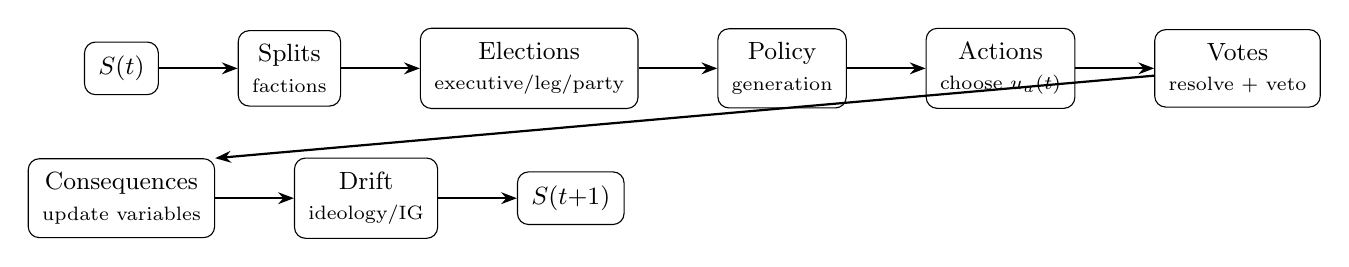
\begin{tikzpicture}[
  box/.style={draw, rounded corners, align=center, font=\small, inner sep=5pt},
  arrow/.style={-{Stealth[length=2mm]}, thick},
]
  \node[box] (s) {$S(t)$};
  \node[box, right=10mm of s] (split) {Splits\\\scriptsize factions};
  \node[box, right=10mm of split] (elect) {Elections\\\scriptsize executive/leg/party};
  \node[box, right=10mm of elect] (pol) {Policy\\\scriptsize generation};
  \node[box, right=10mm of pol] (act) {Actions\\\scriptsize choose $u_a(t)$};
  \node[box, right=10mm of act] (vote) {Votes\\\scriptsize resolve + veto};
  \node[box, below=8mm of s] (cons) {Consequences\\\scriptsize update variables};
  \node[box, right=10mm of cons] (dr) {Drift\\\scriptsize ideology/IG};
  \node[box, right=10mm of dr] (next) {$S(t{+}1)$};
  \draw[arrow] (s) -- (split);
  \draw[arrow] (split) -- (elect);
  \draw[arrow] (elect) -- (pol);
  \draw[arrow] (pol) -- (act);
  \draw[arrow] (act) -- (vote);
  \draw[arrow] (vote) -- (cons.north east);
  \draw[arrow] (cons) -- (dr);
  \draw[arrow] (dr) -- (next);
\end{tikzpicture}
\end{center}

In code (\texttt{src/simulation/engine.py}), a turn is:
\begin{enumerate}
  \item splits and elections (may change roster/roles)
  \item per-place policy generation
  \item per-agent action selection
  \item legislative votes + executive veto + possible override
  \item apply consequences of non-vote actions
  \item ideological drift and IG radicalization/moderation
\end{enumerate}

\section{Action selection model}
\subsection{Action set}
For each agent $a$, an availability filter defines a feasible set of actions
$\mathcal{U}_a(t)$ (see \texttt{src/actions/availability.py}). The decision policy
scores candidates and selects the maximum after adding ambition-scaled Gaussian noise
(\texttt{src/actions/decision.py}).

\begin{center}
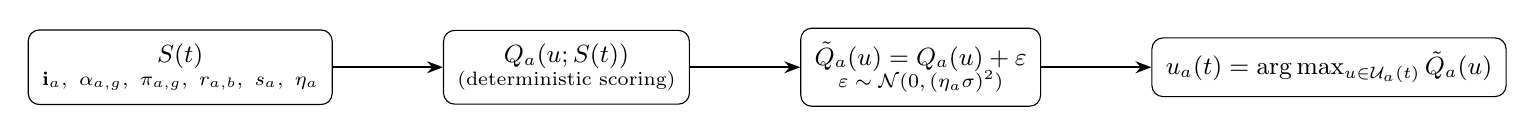
\begin{tikzpicture}[
  box/.style={draw, rounded corners, align=center, font=\small, inner sep=5pt},
  arrow/.style={-{Stealth[length=2mm]}, thick},
]
  \node[box] (state) {$S(t)$\\[-1mm]\scriptsize $\mathbf{i}_a,\ \alpha_{a,g},\ \pi_{a,g},\ r_{a,b},\ s_a,\ \eta_a$};
  \node[box, right=14mm of state] (utility) {$Q_a(u;S(t))$\\[-1mm]\scriptsize (deterministic scoring)};
  \node[box, right=14mm of utility] (noise) {$\tilde Q_a(u)=Q_a(u)+\varepsilon$\\[-1mm]\scriptsize $\varepsilon\sim\mathcal N(0,(\eta_a\sigma)^2)$};
  \node[box, right=14mm of noise] (choice) {$u_a(t)=\arg\max_{u\in\mathcal U_a(t)}\tilde Q_a(u)$};
  \draw[arrow] (state) -- (utility);
  \draw[arrow] (utility) -- (noise);
  \draw[arrow] (noise) -- (choice);
\end{tikzpicture}
\end{center}

\subsection{Utility weights}
Each agent has a weight vector
\[
  \mathbf{w}_a = (w^{pop}_a,w^{stand}_a,w^{ideo}_a,w^{ig}_a,w^{rel}_a),
  \quad \sum_i w_i = 1,
\]
defaulting to \texttt{DEFAULT\_WEIGHTS} in \texttt{src/actions/utility.py}.

\subsection{Noisy argmax decision rule}
For each candidate action $u \in \mathcal{U}_a(t)$ the code forms a deterministic
score $Q_a(u;S(t))$, then adds noise:
\[
  \tilde{Q}_a(u) = Q_a(u;S(t)) + \varepsilon,\qquad
  \varepsilon \sim \mathcal{N}(0, (\eta_a(t)\sigma_u)^2),
\]
with $\sigma_u \in \{0.02,0.01\}$ depending on (agent vs party-leader) action.
Then:
\[
  u_a(t) = \arg\max_{u \in \mathcal{U}_a(t)} \tilde{Q}_a(u).
\]

\section{Voting model}
\subsection{Vote disposition}
When a policy $m$ is put to a vote, each legislator $a \in \mathcal{L}_p(t)$
computes a disposition score $D_a(m) \in [-1,1]$ (see \texttt{compute\_vote\_disposition}
in \texttt{src/actions/voting.py}):
\[
  D_a(m) = \mathrm{clip}_{[-1,1]}\left(
  \sum_{c \in \mathcal{C}} \omega_{a,c}\, v_{a,c}(m)
  \right),
\]
where components $\mathcal{C}=\{\text{ideology, party\_directive, ig\_pressure, electoral, relationships, expulsion\_risk}\}$,
with archetype-conditioned weights $\omega_{a,c}$ (possibly perturbed once per agent and stored).

\begin{center}
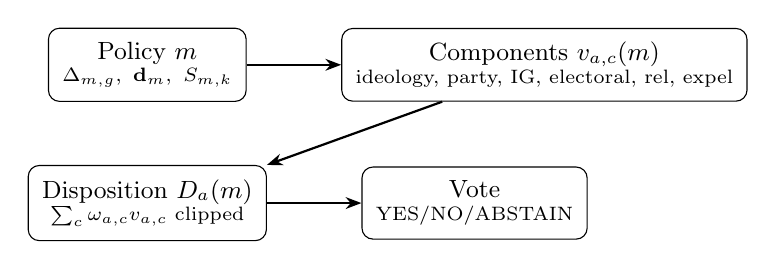
\begin{tikzpicture}[
  box/.style={draw, rounded corners, align=center, font=\small, inner sep=5pt},
  arrow/.style={-{Stealth[length=2mm]}, thick},
]
  \node[box] (policy) {Policy $m$\\[-1mm]\scriptsize $\Delta_{m,g},\ \mathbf d_m,\ S_{m,k}$};
  \node[box, right=12mm of policy] (components) {Components $v_{a,c}(m)$\\[-1mm]\scriptsize ideology, party, IG, electoral, rel, expel};
  \node[box, below=8mm of policy] (disp) {Disposition $D_a(m)$\\[-1mm]\scriptsize $\sum_c \omega_{a,c}v_{a,c}$ clipped};
  \node[box, right=12mm of disp] (vote) {Vote\\[-1mm]\scriptsize YES/NO/ABSTAIN};
  \draw[arrow] (policy) -- (components);
  \draw[arrow] (components) -- (disp.north east);
  \draw[arrow] (disp) -- (vote);
\end{tikzpicture}
\end{center}

\subsection{Component definitions (code-faithful)}
\paragraph{Ideology alignment.}
If $\mathbf{d}_m$ is the policy's axis-direction map and $\mathbf{i}_a$ agent ideology:
\[
  v_{a,\text{ideo}}(m) = \frac{1}{|\mathcal{X}_m|}\sum_{x \in \mathcal{X}_m} i_{a,x}\, d_{m,x}.
\]

\paragraph{Party directive pressure.}
Policies may have an explicit party support scalar $S_{m,k}\in[-1,1]$ stored as
\texttt{policy.attributes["party\_support"][party]}.
Given party threshold $\theta_k$:
\[
  v_{a,\text{party}}(m) =
  \begin{cases}
    \frac{S_{m,k}-\theta_k}{1-\theta_k} & S_{m,k}>\theta_k \\
    \frac{S_{m,k}+\theta_k}{1-\theta_k} & S_{m,k}<-\theta_k \\
    0 & \text{otherwise.}
  \end{cases}
\]

\paragraph{IG pressure.}
Let $\Delta_{m,g}$ be impact and $\alpha_{a,g}$ allegiance. The code dampens low allegiance:
\[
  \alpha'_{a,g} =
  \begin{cases}
    \alpha_{a,g} & \alpha_{a,g}\ge 0.15\\
    0.4\alpha_{a,g} & \alpha_{a,g}<0.15
  \end{cases}
\]
and then
\[
  v_{a,\text{ig}}(m) = \frac{\sum_g \Delta_{m,g}\alpha'_{a,g}}{\sum_g \alpha'_{a,g}}
  \quad (\text{0 if denominator is 0}).
\]

\paragraph{Electoral.}
Popularity-weighted impact:
\[
  v_{a,\text{elect}}(m) = \frac{\sum_g \Delta_{m,g}\pi_{a,g}}{\sum_g \pi_{a,g}}
  \quad (\text{0 if denominator is 0}).
\]

\paragraph{Relationships.}
\[
  v_{a,\text{rel}}(m) = r_{a,\text{proposer}(m)}.
\]

\paragraph{Expulsion risk.}
If directive pressure is $v_{a,\text{party}}(m)\neq 0$, vulnerability in the code is:
\[
  \nu_a = 0.45(1-s_a) + 0.35(1-\bar{\pi}_a) + 0.20(1-\text{altAccess}_a),
\]
clipped to $[0,1]$, and then
\[
  v_{a,\text{expel}}(m)= v_{a,\text{party}}(m)\cdot \nu_a.
\]
(Here $\bar{\pi}_a$ is electorate-share-weighted popularity survivability, and $\text{altAccess}_a$
depends on ideological distance to other parties as in code.)

\subsection{Vote resolution, veto, and override}
Each legislator casts:
\[
  \text{YES if } D_a(m) > 0.1,\quad
  \text{NO if } D_a(m) < -0.1,
\]
else a gray-zone rule that can abstain when personal lean is negative but party pull is positive.

Define indicator functions for each legislator $a \in \mathcal{L}_p(t)$:
\[
  Y_a(m) = \mathbb{I}[D_a(m) > 0.1], \qquad
  N_a(m) = \mathbb{I}[D_a(m) < -0.1].
\]
The bill passes if:
\[
  \sum_{a \in \mathcal{L}_p(t)} Y_a(m) > \frac{1}{2}\,|\mathcal{L}_p(t)|.
\]

If tied (YES=NO) and an executive exists, executive breaks tie in favor iff their $D_{exec}(m)>0$.

If passed, executive vetoes iff $D_{exec}(m) < \tau_p$ where $\tau_p$ is \texttt{gov.veto\_threshold}
(default $-0.3$). Veto override is checked later using a fraction $\phi_p$ (default $2/3$).

\begin{center}
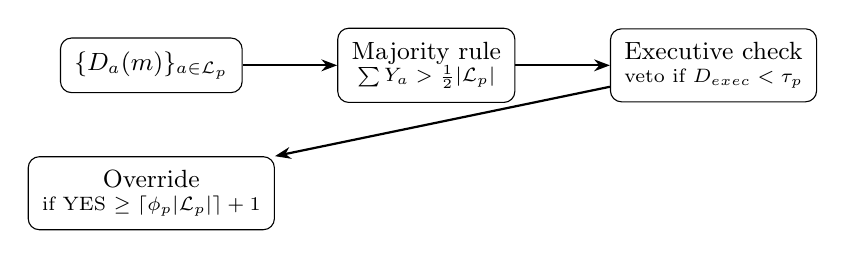
\begin{tikzpicture}[
  box/.style={draw, rounded corners, align=center, font=\small, inner sep=5pt},
  arrow/.style={-{Stealth[length=2mm]}, thick},
]
  \node[box] (votes) {$\{D_a(m)\}_{a\in\mathcal L_p}$};
  \node[box, right=12mm of votes] (pass) {Majority rule\\[-1mm]\scriptsize $\sum Y_a > \frac12|\mathcal L_p|$};
  \node[box, right=12mm of pass] (veto) {Executive check\\[-1mm]\scriptsize veto if $D_{exec}<\tau_p$};
  \node[box, below=8mm of votes] (override) {Override\\[-1mm]\scriptsize if YES $\ge \lceil \phi_p|\mathcal L_p|\rceil+1$};
  \draw[arrow] (votes) -- (pass);
  \draw[arrow] (pass) -- (veto);
  \draw[arrow] (veto) -- (override.north east);
\end{tikzpicture}
\end{center}

\section{Consequences (state updates)}
\begin{center}
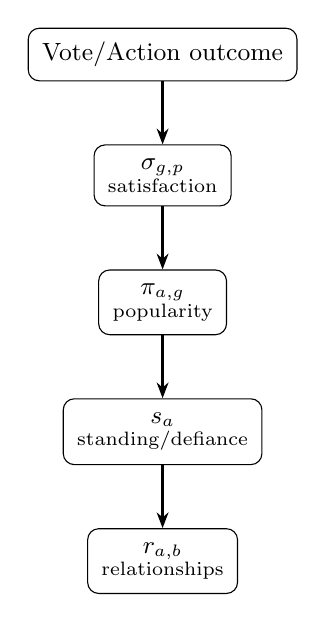
\begin{tikzpicture}[
  box/.style={draw, rounded corners, align=center, font=\small, inner sep=5pt},
  arrow/.style={-{Stealth[length=2mm]}, thick},
]
  \node[box] (outcome) {Vote/Action outcome};
  \node[box, below=8mm of outcome] (ig) {$\sigma_{g,p}$\\[-1mm]\scriptsize satisfaction};
  \node[box, below=8mm of ig] (pop) {$\pi_{a,g}$\\[-1mm]\scriptsize popularity};
  \node[box, below=8mm of pop] (stand) {$s_a$\\[-1mm]\scriptsize standing/defiance};
  \node[box, below=8mm of stand] (rel) {$r_{a,b}$\\[-1mm]\scriptsize relationships};
  \draw[arrow] (outcome) -- (ig);
  \draw[arrow] (ig) -- (pop);
  \draw[arrow] (pop) -- (stand);
  \draw[arrow] (stand) -- (rel);
\end{tikzpicture}
\end{center}

\subsection{Interest-group satisfaction update}
On passage, for each impacted group with satisfaction defined in the place:
\[
  \sigma_{g,p}\leftarrow \mathrm{clip}_{[0,1]}\left(\sigma_{g,p} + \Delta_{m,g}\cdot c(\Delta_{m,g})\right),
\]
where in code $c=0.5$ for $\Delta\ge 0$ and $c=0.6$ for $\Delta<0$ (negatives hit harder).

There is also a cross-IG conflict penalty for pairs of groups with high ideological conflict.

\subsection{Agent popularity update (memory of vote)}
For each voter $a$ and IG $g$:
\[
  \pi_{a,g} \leftarrow \mathrm{clip}_{[0,1]}\left(\pi_{a,g} + \mathrm{dir}(a)\,\Delta_{m,g}\cdot 0.18\right),
\]
where $\mathrm{dir}(a)=+1$ if voted YES else $-1$.

\subsection{Party standing update}
If a party directive is active, following it increases standing; defying decreases it:
\[
  s_a \leftarrow \mathrm{clip}_{[0,1]}(s_a \pm (0.01 + 0.03|v_{a,\text{party}}|) \text{ or } (0.02 + 0.08|v_{a,\text{party}}|)).
\]
The code also tracks \texttt{recent\_defiance}.

\subsection{Relationship update}
Voting together increases mutual trust (+0.02); opposing votes decrease trust (-0.01).
Non-vote actions also adjust relationships and standing (see \texttt{src/simulation/consequences.py}).

\section{Ideological drift and IG radicalization}
\begin{center}
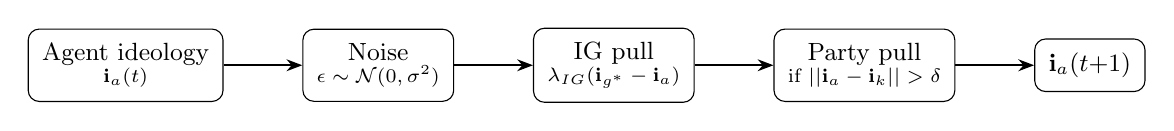
\begin{tikzpicture}[
  box/.style={draw, rounded corners, align=center, font=\small, inner sep=5pt},
  arrow/.style={-{Stealth[length=2mm]}, thick},
]
  \node[box] (agent) {Agent ideology\\[-1mm]\scriptsize $\mathbf i_a(t)$};
  \node[box, right=10mm of agent] (noise) {Noise\\[-1mm]\scriptsize $\epsilon\sim\mathcal N(0,\sigma^2)$};
  \node[box, right=10mm of noise] (igpull) {IG pull\\[-1mm]\scriptsize $\lambda_{IG}( \mathbf i_{g^*}-\mathbf i_a)$};
  \node[box, right=10mm of igpull] (partypull) {Party pull\\[-1mm]\scriptsize if $||\mathbf i_a-\mathbf i_k||>\delta$};
  \node[box, right=10mm of partypull] (next) {$\mathbf i_a(t{+}1)$};
  \draw[arrow] (agent) -- (noise);
  \draw[arrow] (noise) -- (igpull);
  \draw[arrow] (igpull) -- (partypull);
  \draw[arrow] (partypull) -- (next);
\end{tikzpicture}
\end{center}

\subsection{Agent ideology drift}
For each low-detail-level agent and axis $x$ (see \texttt{src/simulation/drift.py}):
\[
  i_{a,x}\leftarrow \mathrm{clip}_{[-1,1]}\Big(
  i_{a,x} + \epsilon_{a,x}
  + \lambda_{IG}(i_{g^*,x}-i_{a,x})
  + \mathbb{1}[|i_{a,x}-i_{k,x}|>\delta]\lambda_{party}(i_{k,x}-i_{a,x})
  \Big),
\]
with $\epsilon_{a,x}\sim\mathcal{N}(0,\sigma^2)$.

\subsection{IG radicalization / moderation}
Let $\bar{\sigma}_g$ be average satisfaction across places.
If $\bar{\sigma}_g < \sigma_{rad}$, the IG becomes more extreme and more mobilized:
\[
  i_{g,x}\leftarrow \mathrm{clip}(i_{g,x}\cdot \gamma + \mathrm{sign}(i_{g,x})\cdot 0.005),\qquad
  e_{g,p}\leftarrow \min(1, e_{g,p}\cdot \kappa).
\]
If $\bar{\sigma}_g > \sigma_{cent}$, it moderates and slightly demobilizes.

\section{Tunable Variables Table (code-extracted)}
The following are the primary \emph{tweak points} exposed as fields or constants in the code.
Some are hard-coded constants; others live in dataclasses and can be changed at initialization time.

\begin{longtable}{@{}p{0.22\linewidth}p{0.18\linewidth}p{0.15\linewidth}p{0.37\linewidth}@{}}
\toprule
\textbf{Variable} & \textbf{Where} & \textbf{Default} & \textbf{Effect} \\
\midrule
\endhead

Turn index $t$ & \texttt{models/world.py} & 0 & Turn counter. \\
Agent ideology $\mathbf{i}_a$ & \texttt{models/agent.py} & --- & Ideological position per axis in $[-1,1]$. \\
IG allegiance $\alpha_{a,g}$ & \texttt{models/agent.py} & \{\} & IG influence weights on agent actions/votes. \\
Agent popularity $\pi_{a,g}$ & \texttt{models/agent.py} & \{\} & IG-specific approval that affects elections/vulnerability. \\
Relationships $r_{a,b}$ & \texttt{models/agent.py} & \{\} & Inter-agent trust used in votes and actions. \\
Party standing $s_a$ & \texttt{models/agent.py} & 0.5 & Loyalty/standing inside party; used in voting/expulsion risk. \\
Ambition $\eta_a$ & \texttt{models/agent.py} & 0.5 & Noise scale for action choice; affects randomness. \\
Utility weights $\mathbf{w}_a$ & \texttt{actions/utility.py} & \texttt{DEFAULT\_WEIGHTS} & Per-agent action utility coefficients. \\
Vote weights $\omega_{a,c}$ & \texttt{actions/voting.py} & (generated) & Per-agent vote component coefficients. \\

Party directive threshold $\theta_k$ & \texttt{models/party.py} & 0.15 & Party-line activation threshold for directives. \\
Campaign budget $B_k$ & \texttt{models/party.py} & 3 & Election nomination budget decrementing on use. \\
Nomination threshold & \texttt{models/party.py} & 0.3 & Minimum nomination score to run a candidate. \\
Leadership interval & \texttt{models/party.py} & 20 & Turns between party leadership elections. \\

Veto threshold $\tau_p$ & \texttt{models/government.py} & -0.3 & Executive veto if exec disposition below threshold. \\
Veto override fraction $\phi_p$ & \texttt{models/government.py} & 2/3 & Fraction of seats needed (plus 1) to override veto. \\
Election interval & \texttt{simulation/elections.py} & --- & Per-government election schedule interval. \\

Default utility weights & \texttt{actions/utility.py} & (0.3,0.2,0.15,0.2,0.15) & Baseline utility weights for action choice. \\

Archetype vote weights & \texttt{actions/voting.py} & varies & Vote-weight baselines by archetype. \\
Vote thresholds & \texttt{actions/voting.py} & $\pm 0.1$ & YES if $>0.1$, NO if $<-0.1$, else gray-zone logic. \\

Drift noise $\sigma$ & \texttt{simulation/drift.py} & 0.01 & Std-dev of per-turn ideology Brownian noise. \\
IG pull rate $\lambda_{IG}$ & \texttt{simulation/drift.py} & 0.02 & Pull rate toward top-allegiance IG ideology. \\
Party pull threshold $\delta$ & \texttt{simulation/drift.py} & 0.4 & Divergence threshold before party-pull activates. \\
Party pull rate $\lambda_{party}$ & \texttt{simulation/drift.py} & 0.015 & Pull rate back toward party ideology. \\
Radicalization threshold $\sigma_{rad}$ & \texttt{simulation/drift.py} & 0.25 & Avg satisfaction below triggers IG radicalization. \\
Radicalization axis scale $\gamma$ & \texttt{simulation/drift.py} & 1.05 & Per-turn multiplier pushing IG ideology away from zero. \\
Radicalization share boost $\kappa$ & \texttt{simulation/drift.py} & 1.02 & Per-turn multiplier increasing IG electorate share. \\
Centrist threshold $\sigma_{cent}$ & \texttt{simulation/drift.py} & 0.72 & Avg satisfaction above triggers IG moderation. \\
Centrist pull rate & \texttt{simulation/drift.py} & 0.03 & Per-turn pull toward 0 for satisfied IG ideology. \\
Centrist share decay & \texttt{simulation/drift.py} & 0.99 & Per-turn multiplier decreasing IG electorate share. \\

Executive term limit & \texttt{simulation/elections.py} & 2 & Default executive term limit if not overridden per agent. \\
Legislative term limit & \texttt{simulation/elections.py} & 4 & Default legislative term limit if not overridden per agent. \\
Stale-agent threshold & \texttt{simulation/elections.py} & 10 & Turns at L2 detail before agent removal. \\
Support dilution factor & \texttt{simulation/elections.py} & 0.25 & Election support dilution (used in election scoring). \\
Viability ratio & \texttt{simulation/elections.py} & 0.6 & Viability cutoff ratio in election mechanics. \\

Split satisfaction threshold & \texttt{simulation/factions.py} & 0.45 & Satisfaction threshold used for faction/split dynamics. \\
Split inertia & \texttt{simulation/factions.py} & 3 & Consecutive-turn inertia required before splitting. \\
Split ideology gap & \texttt{simulation/factions.py} & 0.10 & Minimum ideological gap to justify splinter party. \\
Minimum splinter size & \texttt{simulation/factions.py} & 2 & Minimum members for a new splinter party. \\
Splinter start budget & \texttt{simulation/factions.py} & 2 & Starting campaign budget for newly created parties. \\
Ambition floor & \texttt{simulation/factions.py} & 0.5 & Ambition floor used in split propensity logic. \\

\bottomrule
\end{longtable}

\subsection*{Math $\leftrightarrow$ code mapping}
\begin{longtable}{@{}p{0.22\linewidth}p{0.33\linewidth}p{0.39\linewidth}@{}}
\toprule
\textbf{Math variable} & \textbf{Code} & \textbf{Notes} \\
\midrule
\endhead
$t$ & \texttt{World.turn} & Turn counter. \\
$\mathbf{i}_a$ & \texttt{Agent.ideology.axes} & Ideology by axis name. \\
$\mathbf{i}_k$ & \texttt{Party.ideology.axes} & Party ideology by axis name. \\
$\mathbf{i}_g$ & \texttt{InterestGroup.ideology.axes} & IG ideology by axis name. \\
$\alpha_{a,g}$ & \texttt{Agent.allegiances[InterestGroup]} & Weighted allegiances. \\
$\pi_{a,g}$ & \texttt{Agent.popularity[InterestGroup]} & Popularity per IG. \\
$r_{a,b}$ & \texttt{Agent.relationships[Agent]} & Directed trust edges. \\
$s_a$ & \texttt{Agent.party\_standing} & Party loyalty/standing. \\
$\eta_a$ & \texttt{Agent.ambition} & Action-selection noise scaling. \\
$\mathbf{w}_a$ & \texttt{Agent.attributes["utility\_weights"]} & Defaults to \texttt{DEFAULT\_WEIGHTS}. \\
$\omega_{a,c}$ & \texttt{Agent.attributes["vote\_weights"]} & Seeded from \texttt{ARCHETYPE\_WEIGHTS}. \\
$\sigma_{g,p}$ & \texttt{InterestGroup.satisfaction[Place]} & Satisfaction per place. \\
$e_{g,p}$ & \texttt{InterestGroup.electorate\_share[Place]} & Electorate share per place. \\
$\theta_k$ & \texttt{Party.directive\_threshold} & Directive activation threshold. \\
$B_k$ & \texttt{Party.campaign\_budget} & Used during nominations. \\
$\tau_p$ & \texttt{Government.veto\_threshold} & Executive veto cutoff. \\
$\phi_p$ & \texttt{Government.veto\_override\_fraction} & Override fraction in \texttt{engine.py}. \\
$\sigma$ & \texttt{\_RANDOM\_DRIFT\_SIGMA} & Drift noise in \texttt{simulation/drift.py}. \\
$\lambda_{IG}$ & \texttt{\_IG\_PULL\_RATE} & Drift IG pull. \\
$\delta$ & \texttt{\_PARTY\_PULL\_THRESHOLD} & Party pull threshold. \\
$\lambda_{party}$ & \texttt{\_PARTY\_PULL\_RATE} & Party pull rate. \\
$\sigma_{rad}$ & \texttt{\_RAD\_THRESHOLD} & IG radicalization threshold. \\
$\gamma$ & \texttt{\_RAD\_AXIS\_SCALE} & IG radicalization multiplier. \\
$\kappa$ & \texttt{\_RAD\_SHARE\_BOOST} & IG mobilization multiplier. \\
$\sigma_{cent}$ & \texttt{\_CENTRIST\_THRESHOLD} & IG moderation threshold. \\
\bottomrule
\end{longtable}

\end{document}
